\section{Graph-based Input Representation}
%\label{sec:RelatedWork}

As we mentioned above, the first stage of abstract parsing is static approximation
of relevant string values. Two main representations for approximated values were
used so far. In~\cite{StringExpr,ALVOR1,ALVOR2} the sets of potential string values 
are described using regular expressions; in~\cite{AbstrParsing} approximations are
represented in more implicit form as a solutions of a system of (recursive) dataflow 
equations. 

We did not find a way to scale either of these representations to abstract translation case. 
Instead, we represent the input stream for abstract translation via flow graph with one source and
one sink nodes and string-labeled edges. The labels of edges in this graph represent the results 
of constant propagation so that every path in input graph corresponds to one potential value of dynamic query. 
%Let we define that this path produce corresponded value and we will say that query contains lexical or syntax error if at least 
%one path which produce value with error exists in the corresponding graph. 
Moreover, we perform lexical analysis on graphs which converts the initial string-labeled graphs into
graphs, labeled by tokens.

% After that we define that input graph tokenization or lexical analysis is the process which convert input graph with string labels on edges (Fig.~\ref{pic1}) 
%to graph with tokens. The same way we define parsing or syntax analysis as the process which produce parsing forest by 
%input graph with edges labeled with tokens. As a result of parsing we have forest where each tree corresponds with query 
%value produced by any path in the input graph. When we describe abstract parsing and translation we assume that input 
%graph tokenization performed successfully.

Since any cycle in the input graph generates infinite sequence of tokens which upon translation is turned 
into infinite forest we simplify the graph even more. We replace each cycle with the single repetition. 
Thus the graph becomes cicle-free and we can process all vertices in the topological order.
While this drastic simplification is completely heuristic our experience of dynamic SQL translation 
for real information systems showed that DAG is still a good approximation for practical use.

%In the general case input graph can be arbitrary graph with cycles~\cite{AbstrParsing}. Cycles in the input graph may 
%be cause of infinite parsing. ut we have not found any practice implementations with problem of cycles processing fully 
%solved. We have found only two known implementations of abstract parsing: Alvor\footnote{Alvor is an Eclipse IDE plug-in 
%for statically checking of string-embedded SQL queries in Java programming language. This plug-in is based on LALR and GLR 
%abstract parsing and can be used either for incremental analysis or for offline checking of full code base. Alvor project 
%web site: \href{http://code.google.com/p/alvor/}{http://code.google.com/p/alvor/}} and the tool described in the Doh, Kim, 
%and Schmid's article. Alvor use stack size limitation to avoid infinite processing of cycles. Doh, Kim, and Schmid's 
%implementation of LALR(1)-based abstract parsing cannot be found and article does not contain practice solution of 
%cycles processing problem. In sum, efficient arbitrary graph with cycles processing in abstract parsing is an open question.
	

%For practical usage it is very important that information systems can contain a big 
%number of dynamic queries and each one of them can contains hundreds of 
%branches~\cite{TiunovaUIInt}. The necessity of analyzing all possible values for 
%each query can cause  performance problems and exponential growth of required 
%resources.

As an example consider the following code snippet:

\begin{verbatim} 
   (1) IF @X = @Y
   (2) SET @TABLE = '#tbl1'
   (3) ELSE
   (4) SET @TABLE = 'tbl2'
   (5) SET @S = 'SELECT x FROM ' + @TABLE
   (6) EXECUTE (@S)
\end{verbatim}

Variable \verb @S \ contains dynamically generated query and can have two potential values at the point of query execution. 
During approximation we can build a graph which represents the set of potential values of the variable \verb @S \ at the 
line 6. Each edge of this graph is labeled by a token which represents a part of the query (see Fig.~\ref{pic1}).

\begin{figure}
    \begin{center}
        \includegraphics[width=11cm,height=1.1cm]{graphs/simple_sql.eps}
        \caption{Tokenized input graph}
        \label{pic1}        
    \end{center}
\end{figure}

%Note that real-world systems can 
%communicate with other systems source of which may be inaccessible to analyze. These systems can contain parts of queries 
%to process and we should use some approximations. For example, clients applications of information system can 
%sent conditions for filters (conditions for \verb|where| clause of \verb|select| statement) as part of requests.



